% Báo cáo BTL — smx: Integer-Only Softmax Accelerator
% Biên dịch bằng XeLaTeX (hỗ trợ tiếng Việt và font Times New Roman):
%   cd docs/report && xelatex main.tex && xelatex main.tex

\documentclass[12pt,a4paper]{article}

% ---------- Lề trang ----------
\usepackage[left=3cm,right=2cm,top=2.5cm,bottom=2.5cm]{geometry}

% ---------- Font: Times New Roman (fallback Liberation Serif, cùng metric) ----------
\usepackage{fontspec}
\IfFontExistsTF{Times New Roman}
  {\setmainfont{Times New Roman}}
  {\setmainfont{Liberation Serif}}

% ---------- Cỡ chữ 13pt (class article không có sẵn 13pt) ----------
\makeatletter
\renewcommand\normalsize{%
  \@setfontsize\normalsize{13pt}{16pt}%
  \abovedisplayskip=11pt plus 2pt minus 4pt
  \belowdisplayskip=\abovedisplayskip
}
\makeatother
\normalsize

% ---------- Giãn dòng 1.5, đoạn: before 6pt, after 0 ----------
\usepackage{setspace}
\onehalfspacing
\setlength{\parskip}{6pt}
\setlength{\parindent}{1.25cm}

% ---------- Tiện ích ----------
\usepackage{amsmath}
\usepackage{graphicx}
\graphicspath{{../figures/}}
\usepackage{booktabs}
\usepackage{titlesec}
\usepackage{hyperref}

% Tiêu đề chương (\section) và mục (\subsection)
\titleformat{\section}
  {\normalfont\bfseries\fontsize{13pt}{16pt}\selectfont\centering}
  {Chương \thesection.}{0.5em}{\MakeUppercase}
\titleformat{\subsection}
  {\normalfont\bfseries\fontsize{13pt}{16pt}\selectfont}
  {\thesubsection}{0.5em}{}
\titlespacing*{\section}{0pt}{12pt}{6pt}
\titlespacing*{\subsection}{0pt}{6pt}{0pt}

\begin{document}

% ---------- Trang bìa ----------
\begin{titlepage}
\begin{center}
\textbf{BÁO CÁO BÀI TẬP LỚN}\\[0.3em]
Môn: Cấu trúc phần cứng cho giải thuật học máy\\[0.3em]
Nhóm 6\\[3em]
\textbf{THIẾT KẾ VÀ HIỆN THỰC FPGA BỘ TĂNG TỐC SOFTMAX NGUYÊN THUẦN\\CHO ATTENTION TRANSFORMER}\\[0.3em]
\textit{Design and FPGA Implementation of an Integer-Only Softmax Accelerator for Transformer Attention}\\[4em]
Sinh viên thực hiện: [Họ và tên]\\[1em]
Giảng viên hướng dẫn: [Họ và tên]\\[4em]
Thành phố Hồ Chí Minh, 2026
\end{center}
\end{titlepage}

\tableofcontents
\newpage

\section{Giới thiệu}

\subsection{Bối cảnh}

Cơ chế attention là thành phần cốt lõi của Transformer. Trong mỗi lớp attention, điểm số giữa các vị trí được chuẩn hoá theo hàng bằng hàm softmax trước khi nhân với giá trị. Với độ dài chuỗi $L$, mỗi hàng cần $L$ phép tính $e^{x}$, $L-1$ phép cộng và một phép chia, và điều này lặp lại theo số hàng và số đầu attention. Khi mô hình được lượng tử hoá sang INT8, phần tính softmax trở thành điểm nghẽn nếu vẫn dùng số thực dấu phẩy động.

\subsection{Mục tiêu}

Đề tài xây dựng một bộ tăng tốc softmax theo hàng, trong đó toàn bộ phép tính dùng số nguyên, nhận đầu vào INT8 có dấu và trả về đầu ra UINT8 với scale $1/256$. Bộ tăng tốc được hiện thực dưới dạng IP Avalon-MM slave trên kit DE10-Standard (Cyclone V 5CSXFC6D6F31C6), dùng Quartus Prime Lite 18.1.

Các mục tiêu cụ thể:
\begin{itemize}
  \item Số học bit-exact so với một golden model viết bằng Python.
  \item Tần số hoạt động từ 100 MHz trở lên sau Fitter.
  \item Tổng số ALUT và DSP vượt 1000 theo yêu cầu môn học.
  \item Chạy được trên board qua JTAG và System Console, không cần Linux.
\end{itemize}

\subsection{Phạm vi}

Báo cáo tập trung vào thiết kế lõi \texttt{smx\_core}, gồm thanh ghi điều khiển, bộ đệm X/Y, bộ điều khiển và datapath. Wrapper Avalon, hệ thống Platform Designer và script demo do nhóm hiện thực đảm nhiệm; báo cáo mô tả các phần này ở mức giao diện và cấu trúc hệ thống (Chương 4). Phần kiểm thử lõi do nhóm kiểm thử thực hiện qua cổng \texttt{acc\_*}; kế hoạch và kết quả được trình bày ở Chương 6. Hình \ref{fig:smx-system} cho thấy vị trí của lõi trong hệ thống demo và ranh giới giữa các phần việc.

\begin{figure}[htbp]
  \centering
  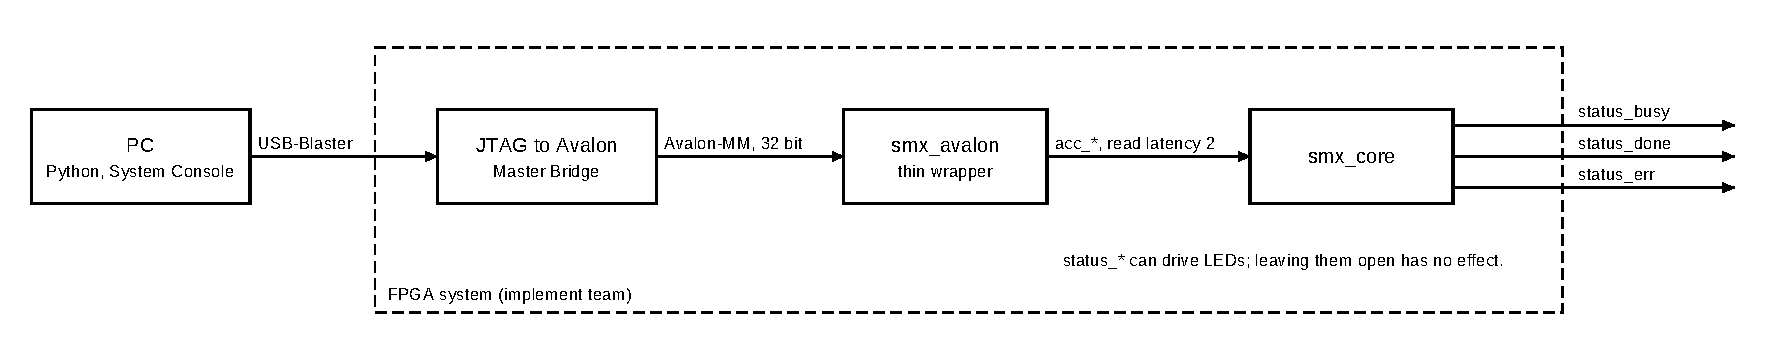
\includegraphics[width=\textwidth]{smx_system.pdf}
  \caption{Ranh giới hệ thống: PC, cầu JTAG to Avalon Master, lớp bao \texttt{smx\_avalon} và lõi \texttt{smx\_core}. Phần trong khung nét đứt nằm trên FPGA.}
  \label{fig:smx-system}
\end{figure}

Đề tài không bao gồm phép nhân ma trận, convolution, LayerNorm, GELU và masking. Hàm sigmoid và GELU chỉ được xem là mở rộng tuỳ chọn sau khi lõi hoàn thành.

\subsection{Đóng góp}

Các đóng góp chính của đề tài gồm:
\begin{enumerate}
  \item Thuật toán softmax thuần số nguyên, không dùng hàm log trong datapath, nhờ đưa hệ số $\log_2 e$ vào $K$ do phần mềm tính sẵn.
  \item Kết hợp IntMax với chuẩn hoá trực tuyến để chỉ cần hai lượt quét và hiệu chỉnh tổng bằng phép dịch.
  \item Tính lại $E$ ở lượt thứ hai từ bộ đệm đầu vào, thay vì lưu kết quả trung gian.
  \item Golden model bit-exact và đặc tả giao diện, làm cơ sở để các nhóm khác tích hợp và kiểm thử.
  \item Lõi RTL đã kiểm thử bit-exact với golden model và đạt mục tiêu tần số, tài nguyên sau Fitter.
\end{enumerate}

\subsection{Tóm tắt kết quả}

Bảng \ref{tab:summary} tóm tắt các kết quả chính của đề tài ở cấu hình mặc định; chi tiết và điều kiện đo nằm ở các chương được dẫn trong bảng.

\begin{table}[htbp]
\centering
\small
\begin{tabular}{lll}
\toprule
Hạng mục & Kết quả & Chương \\
\midrule
Cấu hình mặc định & $P = 8$ lane, $N_{\text{SEG}} = 8$, $L_{\max} = 512$, $R_{\max} = 16$ & 3, 4 \\
Sai số so với softmax float64 & khoảng 0,002, bằng nửa LSB của đầu ra & 3 \\
Tài nguyên sau Fitter & 1\,681 ALUT, 24 DSP, 21 khối M10K & 7 \\
Tần số tối đa & 122 đến 134 MHz qua ba seed & 7 \\
Độ trễ một hàng, $L = 512$ & 182 chu kỳ & 6, 7 \\
Kiểm thử lõi & 7 testcase, 458\,837 phép so, khớp bit-exact & 6 \\
Chạy trên board & [Chưa đo] & 7 \\
\bottomrule
\end{tabular}
\caption{Tóm tắt kết quả chính ở cấu hình mặc định.}
\label{tab:summary}
\end{table}

\subsection{Cấu trúc báo cáo}

Chương 2 khảo sát các hướng softmax phần cứng hiện có. Chương 3 đặc tả thuật toán và số học. Chương 4 mô tả kiến trúc hệ thống và giao diện. Chương 5 trình bày thiết kế từng khối. Chương 6 trình bày kế hoạch và kết quả kiểm thử. Chương 7 trình bày kết quả tổng hợp và đánh giá. Chương 8 kết luận và nêu hướng phát triển.

\section{Cơ sở lý thuyết và khảo sát}

\subsection{Softmax theo hàng}

Với một hàng $x = (x_0, \dots, x_{L-1})$, softmax cho
\begin{equation}
  y_i = \frac{e^{x_i}}{\sum_{k=0}^{L-1} e^{x_k}}, \qquad i = 0, \dots, L-1.
\end{equation}
Để ổn định số học thường trừ đi giá trị lớn nhất trước khi lấy mũ. Trên phần cứng, hai khó khăn chính là hàm mũ và phép chia.

\subsection{Chuẩn hoá trực tuyến}

Milakov và Gimelshein \cite{milakov2018} đề xuất tính max và tổng mũ trong cùng một lượt quét, cập nhật tổng khi max thay đổi bằng hệ số $e^{M_{\text{cũ}}-M_{\text{mới}}}$. Thuật toán này giảm số lượt quét từ ba xuống hai, với điều kiện có cách hiệu chỉnh hệ số đó.

\subsection{Các hướng softmax nguyên thuần}

I-BERT \cite{kim2021ibert} đưa toàn bộ suy luận Transformer về số nguyên, dùng đa thức xấp xỉ cho hàm mũ. Softermax \cite{stevens2021softermax} dùng cơ số 2, max nguyên và PWL cho $2^{F}$. I-ViT và Shiftmax \cite{li2023ivit} dùng dịch bit để hiệu chỉnh hệ số. SoftGen \cite{wei2020softgen} là bộ sinh tham số hoá, cho thấy tính lại phép trừ trên bộ nhớ on-chip giữ diện tích ổn định. SOLE \cite{wang2025sole} và các nghiên cứu log-sum-exp \cite{wang2018lse} khảo sát thêm các dạng xấp xỉ khác.

\subsection{Lựa chọn của đề tài}

Từ khảo sát, đề tài chọn:
\begin{itemize}
  \item Cơ số 2 với hệ số $K = S \cdot \log_2 e$ do phần mềm tính sẵn, nên phần cứng không cần biết $S$ và không cần hàm log.
  \item IntMax để max lấy trên $\lceil u \rceil$, khiến hiệu chỉnh tổng chỉ là phép dịch.
  \item PWL 8 đoạn cho $2^{F}$, đủ để sai số xấp xỉ nằm dưới sai số lượng tử hoá đầu ra.
  \item Một bộ chia tuần tự cho mỗi hàng, mỗi phần tử chỉ một phép nhân.
  \item Tính lại $E$ ở lượt hai từ bộ đệm đầu vào, thay vì lưu trung gian.
\end{itemize}

Chi tiết từng lựa chọn và nguồn gốc số liệu được ghi trong bảng nguồn của tài liệu thiết kế. Các số liệu đo bằng golden model được đánh dấu riêng với các số liệu ước lượng thiết kế.

\section{Đặc tả thuật toán và số học}

Các công thức dưới đây khớp với golden model \texttt{model/softmax\_ref.py}. Khi có mâu thuẫn, golden model là nguồn chân lý.

\subsection{Đầu vào và hệ số $K$}

Đầu vào $q$ là INT8 có dấu. Giá trị thực là $x = S \cdot q$, với $S$ là scale lượng tử hoá của điểm attention. Hệ số
\begin{equation}
  K = \operatorname{round}(S \cdot \log_2 e \cdot 2^{16}),
\end{equation}
là số nguyên không dấu 16 bit (UQ0.16), được phần mềm tính và ghi vào thanh ghi \texttt{SCALE\_K}. Ràng buộc $0 < S < 0{,}693$ để $K$ vừa 16 bit.

\subsection{Số mũ cơ số 2}

Với $u_k = q_k \cdot K$ (25 bit, Q8.16) và $c_k = \lceil u_k / 2^{16} \rceil$ (9 bit có dấu), hàm $E(d)$ với $d \le 0$ được tính như sau. Đặt $I = d \gg 16$, $F = d \,\&\, \text{0xFFFF}$, chỉ số đoạn $\mathit{idx} = F \gg 13$ và phần dư $r = F \,\&\, \text{0x1FFF}$ với $N_{\text{SEG}} = 8$. Khi đó
\begin{align}
  E_0 &= C[\mathit{idx}] + \left((\tilde{M}[\mathit{idx}] \cdot r) \gg 13\right), \\
  E   &= \begin{cases} 0, & -I > 15, \\ E_0 \gg (-I), & \text{ngược lại,} \end{cases}
\end{align}
trong đó $E_0$ là số UQ1.15 16 bit, $C[i] = \operatorname{round}(2^{i/N} \cdot 2^{15})$ và $\tilde{M}[i] = \operatorname{round}((2^{(i+1)/N} - 2^{i/N}) \cdot 2^{15})$. Hai bảng này được sinh bằng \texttt{python3 model/softmax\_ref.py --gen-pwl 8}.

\subsection{Lượt 1: chuẩn hoá trực tuyến với IntMax}

Duyệt các nhóm $g = 0, 1, \dots$ gồm $P = 8$ phần tử liên tiếp theo thứ tự tăng dần. Với nhóm $g$, $M_g = \max_k c_k$. Cập nhật
\begin{align}
  M_{\text{mới}} &= \begin{cases} M_g, & g = 0, \\ \max(M, M_g), & g > 0, \end{cases} \\
  \mathit{sum} &\leftarrow \left(\mathit{sum} \gg (M_{\text{mới}} - M)\right) + \sum_{k \in g} E(u_k - M_{\text{mới}} \cdot 2^{16}), \\
  M &\leftarrow M_{\text{mới}}.
\end{align}
Thứ tự nhóm và phép dịch cắt bỏ là một phần của đặc tả, vì chúng ảnh hưởng đến kết quả bit-exact.

\subsection{Nghịch đảo}

Sau lượt 1, $\mathit{sum} \ge 2^{14}$ và
\begin{equation}
  \mathit{Rcp} = \left\lfloor \frac{2^{40}}{\mathit{sum}} \right\rfloor,
\end{equation}
là số không dấu 27 bit. Phép chia này được thực hiện bằng bộ chia radix-2 tuần tự.

\subsection{Lượt 2: chuẩn hoá đầu ra}

Với mỗi $k < L$, tính lại $e = E(u_k - M \cdot 2^{16})$, trong đó $M$ là giá trị cuối của lượt 1, rồi
\begin{equation}
  y_k = \min\left(255, \; \frac{e \cdot \mathit{Rcp} + 2^{31}}{2^{32}}\right),
\end{equation}
với phép chia là dịch phải số học. Giá trị thực của đầu ra là $y_k / 256$. Trường hợp xác suất bằng 1 không biểu diễn được và được bão hoà về 255.

\subsection{Sai số}

Golden model được kiểm trên hàng ngẫu nhiên $L = 128$ với $S \in \{0{,}02;\, 0{,}0625;\, 0{,}2\}$. Sai số tuyệt đối tối đa so với softmax float64 khoảng $0{,}00195$ đến $0{,}0020$ với $N_{\text{SEG}} = 8$, tức bằng nửa LSB đầu ra. Sai số của xấp xỉ PWL theo số đoạn là $0{,}376\%$, $0{,}094\%$ và $0{,}025\%$ với 4, 8 và 16 đoạn. Với 8 đoạn, sai số xấp xỉ đã nằm dưới sàn lượng tử hoá UINT8, nên lượng tử hoá là yếu tố chi phối.

\subsection{Giới hạn độ dài và độ chính xác}

Độ dài hàng tối đa $L_{\max} = 512$. Số hàng tối đa $R_{\max} = 16$. Các giá trị này xuất hiện trong thanh ghi \texttt{HW\_PARAM} để phần mềm kiểm tra.

\section{Kiến trúc hệ thống}

\subsection{Sơ đồ tổng thể}

Bộ tăng tốc gồm một lõi \texttt{smx\_core} và một lớp bao Avalon-MM mỏng. Lõi chứa toàn bộ thanh ghi điều khiển, bộ đệm đầu vào X, bộ đệm đầu ra Y, bộ điều khiển và datapath. Lõi đưa ra một cổng truy cập bộ nhớ đơn giản \texttt{acc\_*}, có độ trễ đọc cố định 2 chu kỳ và không có tín hiệu chờ.

Luồng dữ liệu của một hàng:
\begin{enumerate}
  \item Lượt 1 đọc $X$ theo nhóm $P$ phần tử, đưa qua phép nhân với $K$, IntMax, $E(d)$ và cây cộng để có $\mathit{sum}$ và $M$.
  \item Bộ chia tính $\mathit{Rcp}$ từ $\mathit{sum}$.
  \item Lượt 2 đọc lại $X$, tính lại $E$, nhân với $\mathit{Rcp}$, làm tròn, bão hoà và ghi vào $Y$.
\end{enumerate}

\subsection{Giao diện}

IP là một Avalon-MM slave với dữ liệu 32 bit và địa chỉ theo word. Giao diện không dùng burst, không dùng \texttt{waitrequest}, và có độ trễ đọc 2 chu kỳ. Phần mềm thăm dò bit \texttt{DONE} để biết khi nào xong; IP không phát ngắt. Ba tín hiệu trạng thái \texttt{status\_busy}, \texttt{status\_done} và \texttt{status\_err} được đưa ra ngoài qua một conduit để nối LED khi demo.

Hai kiểu hệ thống được hỗ trợ:
\begin{itemize}
  \item Đường demo chính: không dùng HPS, master là JTAG to Avalon Master Bridge, điều khiển từ PC bằng System Console.
  \item Đường tuỳ chọn: GHRD Terasic, master là cầu HPS-to-FPGA.
\end{itemize}

\subsection{Bản đồ thanh ghi}

Bảng \ref{tab:regmap} tóm tắt bản đồ thanh ghi, offset tính theo byte.

\begin{table}[htbp]
\centering
\small
\begin{tabular}{lllp{7.2cm}}
\toprule
Offset & Tên & Truy cập & Nội dung \\
\midrule
0x0000 & CTRL      & W   & Bit 0: START (tự xoá) \\
0x0004 & STATUS    & R   & BUSY, DONE, ERR \\
0x0008 & LEN       & R/W & Độ dài hàng $L$, 1..512 \\
0x000C & ROWS      & R/W & Số hàng $R$, 1..16 \\
0x0010 & SCALE\_K  & R/W & Hệ số $K$ (UQ0.16) \\
0x0014 & CYCLE\_CNT & R  & Số chu kỳ từ START đến DONE \\
0x0018 & HW\_PARAM & R   & $P$, $\log_2 L_{\max}$, $R_{\max}$, $\log_2 N_{\text{SEG}}$, VERSION \\
0x2000--0x3FFF & X\_BUF & R/W & INT8, hàng $r$ phần tử $i$ tại byte $r \cdot 512 + i$ \\
0x4000--0x5FFF & Y\_BUF & R   & UINT8, cùng bố trí \\
\bottomrule
\end{tabular}
\caption{Bản đồ thanh ghi của IP (rút gọn từ đặc tả).}
\label{tab:regmap}
\end{table}

\subsection{Trình tự phần mềm}

Phần mềm thực hiện lần lượt các bước sau: tính $K$ và ghi vào \texttt{SCALE\_K}; ghi $R$ hàng vào X\_BUF; ghi \texttt{LEN} và \texttt{ROWS}; ghi START; đọc STATUS cho đến khi DONE bằng 1; đọc Y\_BUF, và đọc CYCLE\_CNT nếu cần đo thời gian.

% Hình minh hoạ: đặt file PDF/SVG trong docs/figures/ rồi bỏ comment.
% \begin{figure}[h]
%   \centering
%   \includegraphics[width=0.9\textwidth]{arch_top.pdf}
%   \caption{Sơ đồ khối tổng thể của smx.}
%   \label{fig:arch}
% \end{figure}

\section{Thiết kế các khối}

Lõi được chia thành mười khối, thiết kế theo thứ tự phụ thuộc. Mỗi khối sẽ có một tài liệu thiết kế riêng và phải được duyệt trước khi viết RTL. Trạng thái tại thời điểm viết báo cáo được tóm tắt trong Bảng \ref{tab:blocks}.

\begin{table}[h]
\centering
\begin{tabular}{clll}
\toprule
\# & Khối & Vai trò & Trạng thái \\
\midrule
1  & \texttt{smx\_exp2}    & $d \to E$, PWL và dịch & TODO \\
2  & \texttt{smx\_scale}   & $u = q \cdot K$, $c = \lceil u \rceil$ & TODO \\
3  & \texttt{smx\_maxtree} & $M_g$ và cập nhật $M$ & TODO \\
4  & \texttt{smx\_sumacc}  & Cây cộng và tích luỹ có dịch & TODO \\
5  & \texttt{smx\_divider} & $\lfloor 2^{40} / \mathit{sum} \rfloor$ tuần tự & TODO \\
6  & \texttt{smx\_norm}    & $E \cdot \mathit{Rcp}$, làm tròn, bão hoà & TODO \\
7  & \texttt{smx\_buf}     & Hai bank 32 bit, byte-enable & TODO \\
8  & \texttt{smx\_csr}     & Thanh ghi, START/DONE/ERR & TODO \\
9  & \texttt{smx\_ctrl}    & FSM hàng và lượt & TODO \\
10 & \texttt{smx\_core}    & Nối các khối & TODO \\
\bottomrule
\end{tabular}
\caption{Danh sách khối và trạng thái thiết kế.}
\label{tab:blocks}
\end{table}

\subsection{Khối số học}

Khối \texttt{smx\_exp2} là khối phức tạp nhất về số học, vì phải khớp bit-exact với bảng PWL và phép dịch. Khối \texttt{smx\_sumacc} nằm trên đường găng về timing vì có vòng phản hồi qua $M$ và $\mathit{sum}$. Khối \texttt{smx\_divider} là bộ chia tuần tự radix-2, ước lượng khoảng 28 chu kỳ mỗi hàng.

\subsection{Khối lưu trữ và điều khiển}

Hai bộ đệm X và Y dùng chung một module \texttt{smx\_buf}, mỗi bộ gồm hai bank 32 bit $\times$ 1024. Khối \texttt{smx\_ctrl} điều khiển thứ tự hàng, lượt, địa chỉ và mặt nạ lane.

\subsection{Kết quả thiết kế}

Chưa có kết quả RTL và mô phỏng tại thời điểm viết báo cáo. Các số liệu tài nguyên và độ trễ sẽ được điền sau khi có báo cáo từ Quartus và mô phỏng thật.

\section{Kế hoạch kiểm thử}

\subsection{Golden model làm scoreboard}

Golden model \texttt{softmax\_row} là chuẩn so sánh. Mọi kết quả RTL phải khớp bit-exact trên từng hàng. Vector kiểm thử được sinh từ golden model và lưu trong thư mục \texttt{tb/vectors/}.

\subsection{Kịch bản tối thiểu}

Các kịch bản bắt buộc gồm:
\begin{itemize}
  \item Độ dài $L = 1$, $L = P$, $L = P \pm 1$ và $L = L_{\max}$.
  \item Số hàng $R = 1$ và $R = R_{\max}$.
  \item Hệ số $K = 0$, $K = 1$ và $K = 65535$.
  \item Hàng toàn $-128$, toàn $127$, đồng nhất, và one-hot ở cực trị.
  \item Hàng có max nằm ở nhóm cuối, để kiểm tra phép dịch hiệu chỉnh.
  \item Vector ngẫu nhiên.
\end{itemize}

\subsection{Khẳng định}

Các khẳng định đề xuất cho nhóm verification gồm: lệnh START khi BUSY bị bỏ qua; DONE chỉ lên sau khi BUSY xuống; LEN hoặc ROWS ngoài khoảng làm ERR lên; không có X hoặc Z trên đường đọc khi \texttt{readdatavalid}.

\subsection{Kết quả kiểm thử}

Chưa có kết quả mô phỏng tại thời điểm viết báo cáo. Kết quả từng khối sẽ được ghi sau khi unit test chạy trên ModelSim hoặc Questa.

\section{Tổng hợp và đánh giá}

\subsection{Mục tiêu đánh giá}

Đánh giá gồm bốn nhóm số liệu: tài nguyên (ALUT, DSP, M10K), tần số tối đa (Fmax), độ trễ mỗi hàng và số chu kỳ đo được qua \texttt{CYCLE\_CNT}. Ngoài ra có thể quét tham số $P$ và $N_{\text{SEG}}$.

\subsection{Tài nguyên và tần số}

\begin{table}[h]
\centering
\begin{tabular}{lll}
\toprule
Chỉ số & Mục tiêu & Kết quả \\
\midrule
ALUT + DSP   & $> 1000$ & [Chưa đo] \\
Số DSP       & 12--24   & [Chưa đo] \\
Fmax         & $\ge 100$ MHz & [Chưa đo] \\
Độ trễ mỗi hàng ($L = 512$, $P = 8$) & $\le 192$ chu kỳ & [Chưa đo] \\
\bottomrule
\end{tabular}
\caption{Mục tiêu và kết quả tổng hợp (điền sau khi có báo cáo Quartus).}
\label{tab:synth}
\end{table}

\subsection{Quét tham số}

Mục tiêu quét gồm $P \in \{4, 8, 16\}$ và $N_{\text{SEG}} \in \{4, 8, 16\}$, cùng độ dài $L$ thay đổi. Kết quả sẽ được trình bày bằng bảng và đồ thị lưu trong \texttt{docs/figures/}.

\subsection{Đánh giá ban đầu}

Các số liệu về sai số đã có từ golden model, được nêu ở Chương 3. Các số liệu về tài nguyên, tần số và độ trễ chỉ là ước lượng thiết kế và sẽ được thay bằng số đo thật.

\section{Kết luận và hướng phát triển}

\subsection{Kết luận}

Đề tài đã xây dựng thuật toán softmax thuần số nguyên cho attention, với đặc tả số học bit-exact, golden model làm chuẩn so sánh và giao diện đóng băng ở phiên bản 1.0. Việc chọn cơ số 2, IntMax, PWL 8 đoạn và tính lại $E$ ở lượt hai giúp datapath không cần hàm log và chỉ có một phép chia mỗi hàng.

Lõi \texttt{smx\_core} đã được hiện thực bằng SystemVerilog và tích hợp đủ mười khối. Trong mô phỏng, lõi khớp bit-exact với golden model trên toàn bộ bảy testcase của nhóm kiểm thử, với $P \in \{4, 8, 16\}$ và $N_{\text{SEG}} \in \{4, 8, 16\}$. Sau Fitter ở $P = 8$, lõi dùng 1\,681 ALUT, 24 DSP và 21 khối M10K, đạt từ 122 MHz trở lên qua ba seed, và xử lý một hàng 512 phần tử trong 182 chu kỳ.

\subsection{Hướng phát triển}

Lớp bao Avalon-MM, thành phần Platform Designer và hệ thống demo cho kit DE10-Standard đã được viết và biên dịch thành công, nhưng chưa chạy trên board. Các việc tiếp theo gồm: đối chiếu gán chân, nạp thiết kế lên board và điều khiển qua System Console; kiểm thử ở mức bus Avalon; chạy Fitter cho $N_{\text{SEG}} = 4$ và 16 và thêm seed ở $P = 4$; ràng buộc timing cho cổng \texttt{acc\_*}; đánh giá độ chính xác của toàn mạng trên mô hình mục tiêu bằng golden model. Mở rộng tuỳ chọn gồm masking và các hàm sigmoid, GELU.


\begin{thebibliography}{99}

\bibitem{milakov2018}
M.~Milakov and N.~Gimelshein. Online normalizer calculation for softmax. 2018.

\bibitem{kim2021ibert}
S.~Kim et al. I-BERT: Integer-only BERT quantization. ICML, 2021.

\bibitem{stevens2021softermax}
J.~R.~Stevens et al. Softermax: Hardware/software co-design of an efficient softmax for transformers. DAC, 2021.

\bibitem{li2023ivit}
Z.~Li and Q.~Gu. I-ViT: Integer-only quantization for efficient vision transformer inference. ICCV, 2023.

\bibitem{wei2020softgen}
X.~Wei et al. SoftGen: Hardware generator for softmax. ASAP, 2020.

\bibitem{wang2018lse}
Z.~Wang et al. Log-sum-exp hardware approximation. APCCAS, 2018.

\bibitem{wang2025sole}
Wang et al. SOLE: Hardware-software co-design of softmax and layer normalization for transformers. 2025.

\end{thebibliography}


\end{document}
